
\chapter{System Capability Analysis}
\label{sec:capability_analysis}

% Chebychev inequality for failure probability and other measures of inequality. Important! + confidence intervals
% slope of qq plot
% goodness of fit tests
% Robust version of C_p (without the in-control assumption)


In a system capability analysis, we essentially use statistical tools to measure the variability in a production process.
This analysis can answer questions that are raised at the measuring, analyzing, and improving stages of the DMAIC cycle. 
The methods we will discus compare between the processes variability and specification. 
Note, however, that a simple statistical analysis of the production process, without relating to specification, may also be qualify as a system capability analysis.

We naturally want production processes that adhere to specifications, and want to quantify the level of adherence.
The quantification is performed by comparing the variability in a CTQ to the specification.
In this chapter we assume the process’s capability is fixed over time. 
In Chapter~\ref{sec:advanced_capability_analysis} we revisit the same problems, when allowing the process’s capability to vary over time. 

The particular setup discusses in this chapter is also known as \emph{product specification}.\marginnote{Product Specification}
When we use the actual time, and ordering of data samples, as in a control chart, we will no longer regard it as product specification but rather as a bona-fide capability analysis. This is the subject of Chapter~\ref{sec:advanced_capability_analysis}.
 
 
\section{Specification Agnostic Capability Analysis}
 
Because capability analysis, or product specification, is essentially the study of the CTQ's distribution, it can be approached with the aforementioned statistical tools such as univariate summary statistics and visualizations presented in Sections~\ref{sec:summary_statistics} and \ref{sec:visualizations}.
If particular hypothesis want to be tested on the distribution of the CTQ, we may call upon the inference tools from Chapter~\ref{sec:inference}.

\section{Specification Aware Capability Analysis}
Classical statistical devices are not aimed at introducing the designed process's capabilities.
We will thus introduce several measures that do so, collectively called \emph{process capability ratios} (PCR), or \emph{process capability index}.\marginnote{Process Capability Index}
The first, and most basic PCR is the $\cp$ of a particular CTQ.

\begin{definition}[$\cp$]
\begin{align}
\label{eq:cp}
	C_p:= \frac{USL-LSL}{6 \sigma}, 
\end{align}
where $\sigma$ is the standard deviation of the CTQ.

\end{definition}
Clearly $\cp$ is a process parameter, that needs to be estimated.
\begin{definition}[$\cpHat$]
\begin{align}
	\cpHat:= \frac{USL-LSL}{6 \hat{\sigma}}, 
\end{align}
where $\hat{\sigma}$ is some estimate of the standard deviation of the CTQ.
\end{definition}
The most natural $\hat{\sigma}$ is the sample standard deviation $s$, but we will explore other options in the following.


There is a relation between $C_p$ and the probability of non-conformance. 
To explore this relation we introduce the following notation, under the assumption of a symmetric specification about its target value.
\begin{tcolorbox}
\footnotesize
\textbf{Collecting Notation} \newline
$\targetValue:= (USL+LSL)/2$, the target value. \newline
$\delta:= (USL-LSL)/2$.  \newline
$\ctqExpect:= \expect{CTQ}$, the expected CTQ. \newline
$1-\pnc:= P(CTQ \in [LSL,USL])$, the probability of compliance, thus $\pnc$ is the probability of non compliance. 
\end{tcolorbox}

With our new notation Eq.(\ref{eq:cp}) is now $\cp=\frac{\delta}{3 \sigma}$.
Assuming $CTQ \sim \gauss{\mu, \sigma^2}$, and that the process is centred so that $\ctqExpect=\targetValue$, then $\cp$ is related to $\pnc$ via
\begin{align}
\label{eq:pc_and_pnc}
 \pnc= 2\, \Phi(-3 \cp)
\end{align}
As a sanity check, we check this relation for a 3-sigma process.
A 3-sigma process implies that $\cp=1$, and Eq.(\ref{eq:pc_and_pnc}), implies that $\pnc=0.0027$, as we have already seen in six-sigma introduction in Section~\ref{sec:six_sigma}.

To derive Eq.(\ref{eq:pc_and_pnc}) we had to call upon several assumptions.
Namely:
\begin{enumerate}
\item The CTQ has a normal distribution.
\item The process is in statistical control, i.e. $\ctqExpect$ is fixed over time
\item The process is centered, i.e. $\ctqExpect=\targetValue$.
\item $\targetValue$ is mid-way between LSL and USL.
\end{enumerate}








\subsection{Non-Conformance for a Non-Gaussian CTQ}
The first assumption we will now relax is the Gaussianity of $CTQ$. 

\begin{theorem}[Chebyshev's inequality]
For any random variable $\x$, with $\mu:=\expect{\x}$, and $\sigma^2:=\expect{(\x-\mu)^2}$, then
\begin{align}
	P(|\x-\mu|>k\sigma)=\frac{1}{k^2}
\end{align}
\end{theorem}
An immediate application of Chebyshev's inequality yields that for \emph{any} distribution of the CTQ, then $\pnc<0.11$.
This is nice, but far from amazing, since it means that a 3-sigma process, assumingly with $2,700 ppm$, may actually have $111,111 ppm$, if we were wrong about the Gaussianity assumption.
We now present a similar bound on $\pnc$ that applies to all \emph{unimodal} CTQ distributions.

\begin{theorem}[Vysochanskij–Petunin inequality]
For any random variable $\x$, with $\mu:=\expect{\x}$, $\sigma^2:=\expect{(\x-\mu)^2}$, with unimodal distribution, and for $k>\sqrt{8/3}=1.63299$, then 
\begin{align}
	P(|\x-\mu|>k\sigma)=\frac{4}{9 k^2}
\end{align}
\end{theorem}
Since $3$ is obviously larger than $1.63299$, then an immediate application of Vysochanskij–Petunin inequality yields that for a unimodal CTQ, then $\pnc<0.0493$, or $49,383 ppm$.
Again we see that if we wrongly assumed normality, we may have many more non-compliances than we thought. Then again, both Chebyshev and Vysochanskij–Petunin are very loose bounds. 
They should thus be seen as a worst-case, while reality is not as bad.

Another important approach to dealing with non-Gaussianity of the CTQ is by a non-linear change of scale.
As  a rule of thumb, you may try scale transformation such as a log-transform and a square-root, and then inspect the normality of the data with the tools discusses in Chapters~\ref{sec:exploratory} and \ref{sec:inference}.

We now consider $\cpHat$, i.e., the estimation of $\cp$.
For a Gaussian CTQ, then $\sigma$ can naturally be estimated by $s$. 
If, however, the Gaussianity assumption does not hold, even if the process is under control, then $s$ may be a poor estimator of $\sigma$.
We may now recall that in Chapter~\ref{sec:exploratory} we encountered several measure of scale such as the IQR (Definition~\ref{def:iqr}), and MAD (Definition~\ref{def:mad}).
Since $s$ is essentially a measure of scale, we may replace $s$ by the IQR, or the MAD, for example, and still retain a valid estimator of $\cp$.








\subsection{Process Capability of a non-centred Process}
We will now relax the assumption of $\ctqExpect=\targetValue$, while still in statistical control.

\begin{definition}[$\cpk$]
\begin{align}
	\cpk:= \min\set{\cpu,\cpl}
\end{align}
where $\cpu:= \frac{USL- \ctqExpect}{3 \sigma}$ and $\cpl:= \frac{\ctqExpect-LSL}{3 \sigma}$.
\end{definition}
For a non-centered process, this definition is more informative on the probability of non-compliance.
Generally, $\cpk \leq \cp$, with equality holding under statistical control ($\ctqExpect=\targetValue$).
An illustration is given in Figure~\ref{fig:cpk}.

\begin{figure}
\centering
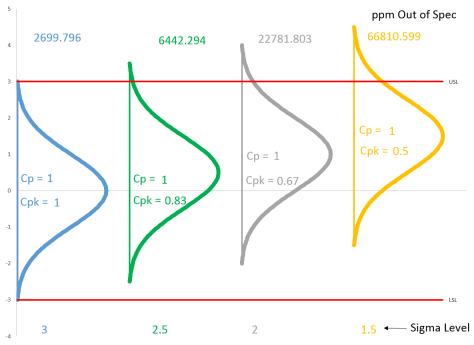
\includegraphics[height=0.3\textheight]{art/Cpk_same_sigma_varying_avg}
\caption[$\cpk$ and $\cp$]{$\cpk$ and $\cp$. \newline
\url{https://www.spcforexcel.com/knowledge/process-capability/interactive-look-process-capability}.}
\label{fig:cpk}
\end{figure}

